%!TEX program = xelatex
\documentclass{beamer}

% Correct the path when including svg pictures
\RequirePackage{import}

% To resize graphic and table
\RequirePackage{graphics}

% For nice verbatim
\RequirePackage{minted}

% Arrange theme
\usetheme[
	progressbar=frametitle,
	sectionpage=none,
	numbering=fraction
]{metropolis}

% Color the progress:
% - green for SciLifeLab
% - violet for KI
\setbeamercolor{progress bar}{fg=violet,bg=white}

\author{Maxime Garcia}
\date{2017-08-29}
\title{Cancer Analysis Workflow}
\titlegraphic{\hfill
\includegraphics[height=1cm]{pictures/CAW}}
\subtitle{Yes we can run it on Irma with Singularity containers}
\institute{% Don't forget logos
	\vfill
	
\includegraphics[height=.7cm]{pictures/SciLifeLab}
	\hfill
	
\includegraphics[height=.7cm]{pictures/NGI}
	\hfill
	
\includegraphics[height=.7cm]{pictures/NBIS}
	\hfill
	
\includegraphics[height=.7cm]{pictures/KI}
	\hfill
	
\includegraphics[height=.7cm]{pictures/KTH}
	\hfill
	
\includegraphics[height=.7cm]{pictures/SU}
	\hfill
	
\includegraphics[height=.7cm]{pictures/UU}
	\hfill
	
\includegraphics[height=.7cm]{pictures/Barntumorbanken}
}

\begin{document}

\maketitle

\section{Singularity}

\begin{frame}{What is Singularity?}
	\vspace{-2cm}
	\center{
\includegraphics[height=2cm]{pictures/singularity.png}}
	\begin{itemize}
		\item Docker-like containers technology
		\item Specific for HPC environnment
		\pause
		\item Without the root user security problem
		\pause
		\item Supported by Nextflow
		\pause
		\item Can pull containers from Docker-hub
	\end{itemize}
\end{frame}

\section{Motivation}

\begin{frame}{Why would we want to do that?}
	\begin{itemize}
		\item For a better control
		\pause
		\item of every tool used
		\item of every version used
		\pause
		\item For a better reproducibility
		\pause
		\item Containerization is reproducible and portable
	\end{itemize}
\end{frame}

\begin{frame}{We can do everything!}
	\center{
\includegraphics[height=7.5cm]{pictures/Penguin-meme.png}}
\end{frame}

\section{CAW-containers}

\begin{frame}{The CAW-containers repository}
	\center{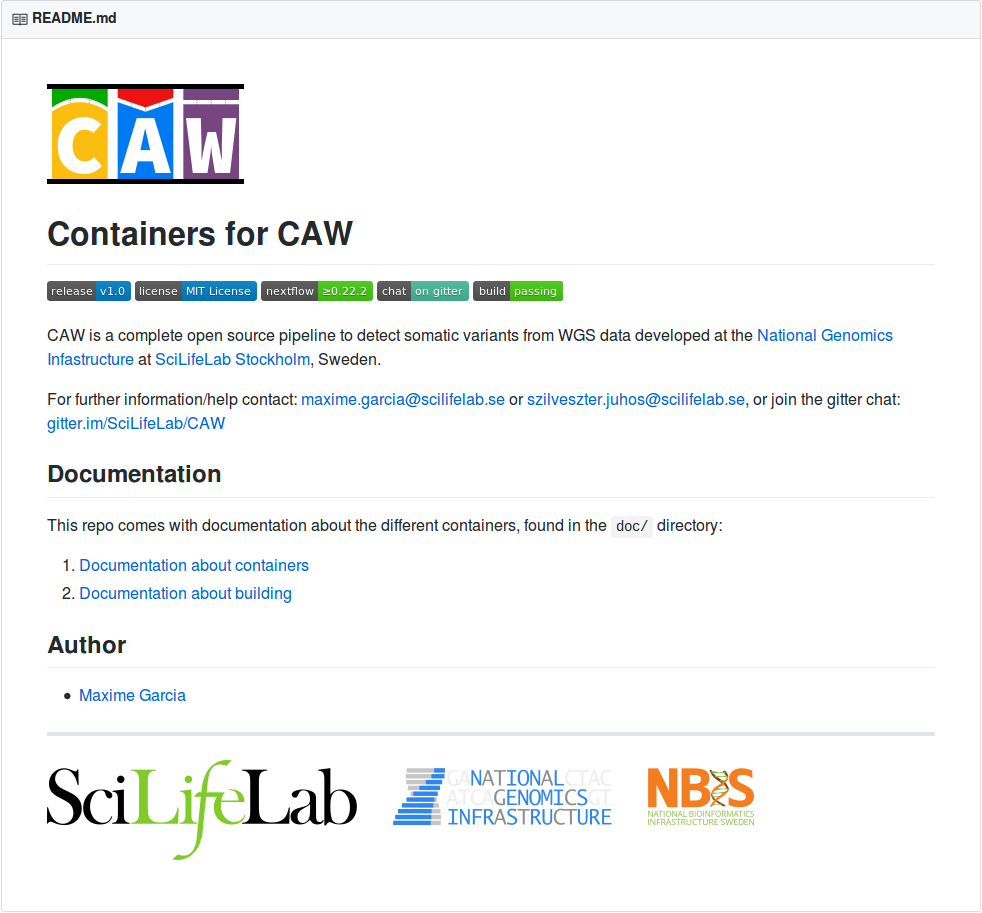
\includegraphics[height=7.5cm]{pictures/CAW-containers.png}}
\end{frame}

\begin{frame}{The One Script}
	\mint[fontsize=\small]{html}|SciLifeLab/CAW-containers|
	\begin{itemize}
		\item 24 different Docker containers for all the different processes
		\pause
		\item One Script to build them all,
		\pause
	\end{itemize}
	\hfill One Script to push them \hspace{1.5cm}
	\pause
	\begin{itemize}
		\item One Script to pull them all,
	\end{itemize}
	\pause
	\hfill and with Singularity run them \hspace{1.5cm}
\end{frame}

\begin{frame}[fragile]{Inside the script}
\mint[fontsize=\small]{html}|SciLifeLab/CAW-containers/main.nf|
\begin{minted}[fontsize=\scriptsize]{text}
docker build -t $repository/$container:$tag \
  $baseDir/containers/$container/.

docker push $repository/$container:$tag

singularity pull --name $container-${tag}.img \
  docker://$repository/$container:$tag
\end{minted}
\end{frame}

\section{Usage with Nextflow}

\begin{frame}{Nextflow and Singularity for the win}
	\vspace{-3cm}
	\center{
\includegraphics[height=1cm]{pictures/nextflow.png}}
	\begin{itemize}
		\item Nextflow natively support Singularity
		\pause
		\item Easy configuration
		\pause
		\item Automatic pull of the containers
	\end{itemize}
\end{frame}

\begin{frame}[fragile]{Easy configuration}
\mint[fontsize=\scriptsize]{html}|SciLifeLab/CAW/configuration/singularity.config|
\begin{minted}[fontsize=\scriptsize]{text}
singularity {
  autoMounts = true
  enabled = true
}
process {
  $RunFastQC.container        = 'docker://maxulysse/fastqc:1.1'
  $RunFreeBayes.container     = 'docker://maxulysse/freebayes:1.1'
  $RunGenotypeGVCFs.container = 'docker://maxulysse/gatk:1.1'
  $RunManta.container         = 'docker://maxulysse/runmanta:1.1'
  $RunMultiQC.container       = 'docker://maxulysse/multiqc:1.1'
  $RunMutect1.container       = 'docker://maxulysse/mutect1:1.1'
}

\end{minted}
\pause
\begin{minted}[fontsize=\scriptsize]{text}
process.container = 'shub://MaxUlysse/shubcontainer'
\end{minted}
\end{frame}

\begin{frame}{What to do on a secure cluster?}
	\begin{itemize}
		\item How about running CAW with Singularity on Bianca or Irma?
		\pause
		\item No automatic pull of the containers
		\pause
		\item The configuration is still easy
	\end{itemize}
\end{frame}

\begin{frame}[fragile]{Still an easy configuration}
	\mint[fontsize=\scriptsize]{html}|SciLifeLab/CAW/configuration/singularity-download.config|
\begin{minted}[fontsize=\scriptsize]{text}
singularity {
  autoMounts = true
  enabled = true
}
process {
  $RunFastQC.container        = 'containers/fastqc-1.1.img'
  $RunFreeBayes.container     = 'containers/freebayes-1.1.img'
  $RunGenotypeGVCFs.container = 'containers/gatk-1.1.img'
  $RunManta.container         = 'containers/runmanta-1.1.img'
  $RunMultiQC.container       = 'containers/multiqc-1.1.img'
  $RunMutect1.container       = 'containers/mutect1-1.1.img'
}
\end{minted}
\end{frame}

\begin{frame}{How to get the containers?}
	\begin{itemize}
		\item Use the script that does the thing
		\pause
		\item To pull all containers from Docker-hub into Singularity containers
		\pause
		\item Transfer the containers to the secure cluster
	\end{itemize}
\end{frame}

\begin{frame}{One last detail}
	\begin{itemize}
		\item Do not forget to create the UPPMAX specific directories in the containers
		\pause
		\item \mint{text}|/pica|
		\pause
		\item \mint{text}|/proj|
		\pause
		\item \mint{text}|/sw|
	\end{itemize}
\end{frame}


\begin{frame}[fragile]{Let the magic happen}
\mint[fontsize=\small]{html}|SciLifeLab/CAW/main.nf|
\begin{minted}[fontsize=\scriptsize]{text}
nextflow run ~/CAW/main.nf --project project --step preprocessing \
  --genome GRCh38 --sample sample.tsv -profile singularityLocal
\end{minted}
\end{frame}

\section{What about TravisCI?}

\begin{frame}[fragile]{Using parralelization to do multiple tests}
\mint[fontsize=\small]{html}|SciLifeLab/CAW/.travis.yml|
\begin{minted}[fontsize=\tiny]{text}
	sudo: required
	language: java
	jdk: openjdk8
	services:
	  - docker
	env:
	  - NXF_VER=0.25.6 SGT_VER=2.3.1 TEST=ANNOTATE PROFILE=singularity
	  - NXF_VER=0.25.6 SGT_VER=2.3.1 TEST=ANNOTATE PROFILE=docker
	  - NXF_VER=0.25.6 SGT_VER=2.3.1 TEST=RECALIBRATE PROFILE=singularity
	  - NXF_VER=0.25.6 SGT_VER=2.3.1 TEST=RECALIBRATE PROFILE=docker
	  - NXF_VER=0.25.6 SGT_VER=2.3.1 TEST=REALIGN PROFILE=singularity
	  - NXF_VER=0.25.6 SGT_VER=2.3.1 TEST=REALIGN PROFILE=docker
	  - NXF_VER=0.25.6 SGT_VER=2.3.1 TEST=MAPPING PROFILE=singularity
	  - NXF_VER=0.25.6 SGT_VER=2.3.1 TEST=MAPPING PROFILE=docker

	install: # Install Nextflow
	  - "./scripts/install.sh --tool nextflow"

	script:
	  - "./scripts/test.sh --profile $PROFILE --test $TEST --install --travisci"
\end{minted}
\end{frame}

\begin{frame}{All your test are belong to us.}
	\center{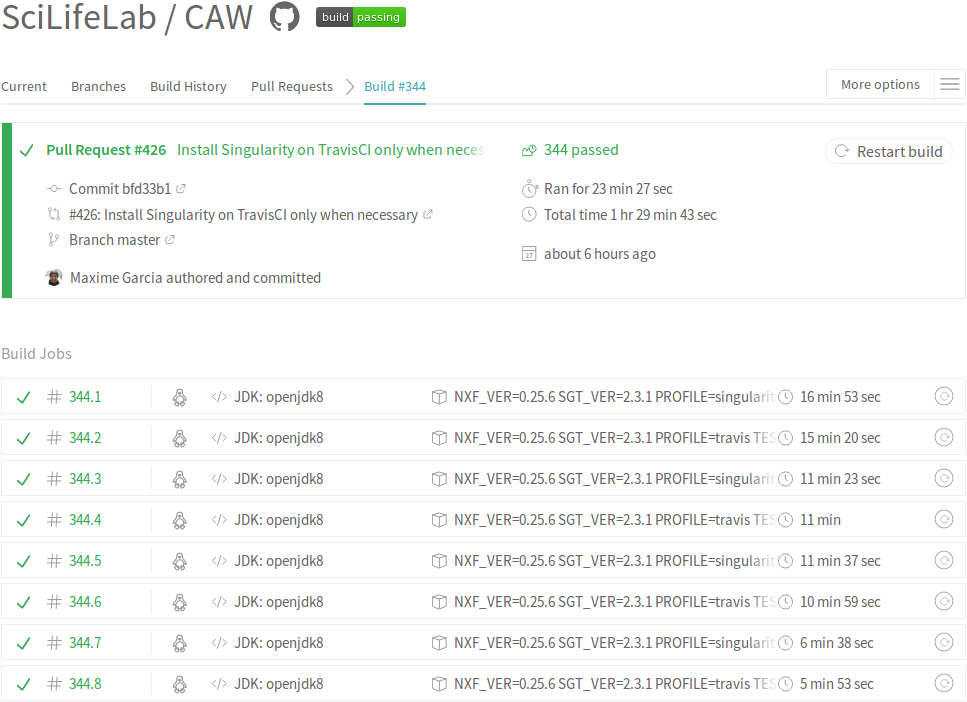
\includegraphics[height=7.5cm]{pictures/Travis.png}}
\end{frame}


\section{Acknowledgements}

\begin{frame}{The List of People Involved}
	\begin{table}
		\resizebox{.4\textwidth}{!}{%
		\begin{tabular}{l}
			Sebastian DiLorenzo \\
			Jesper Eisfeldt \\
			Maxime Garcia \\
			Szilveszter Juhos \\
			Max Käller \\
			Malin Larsson \\
			Marcel Martin \\
			Monica Nistèr \\
			Björn Nystedt \\
			Pall Olason \\
			Pelin Sahlén \\
			Johanna Sandgren \\
			Teresita Díaz De Ståhl \\
		\end{tabular}}
	\end{table}
\end{frame}

\begin{frame}[fragile]{Where to find us?}
	\begin{itemize}
		\item We are on the SciLifeLab Slack
		\mint[fontsize=\small]{html}|#cancer-pipeline|
		\pause
		\item We have a gitter channel
		\mint[fontsize=\small]{html}|https://gitter.im/SciLifeLab/CAW|
		\pause
		\item Our code is hosted on Github
		\mint[fontsize=\small]{html}|https://github.com/SciLifeLab/CAW|
	\end{itemize}
\end{frame}

\usebackgroundtemplate{
	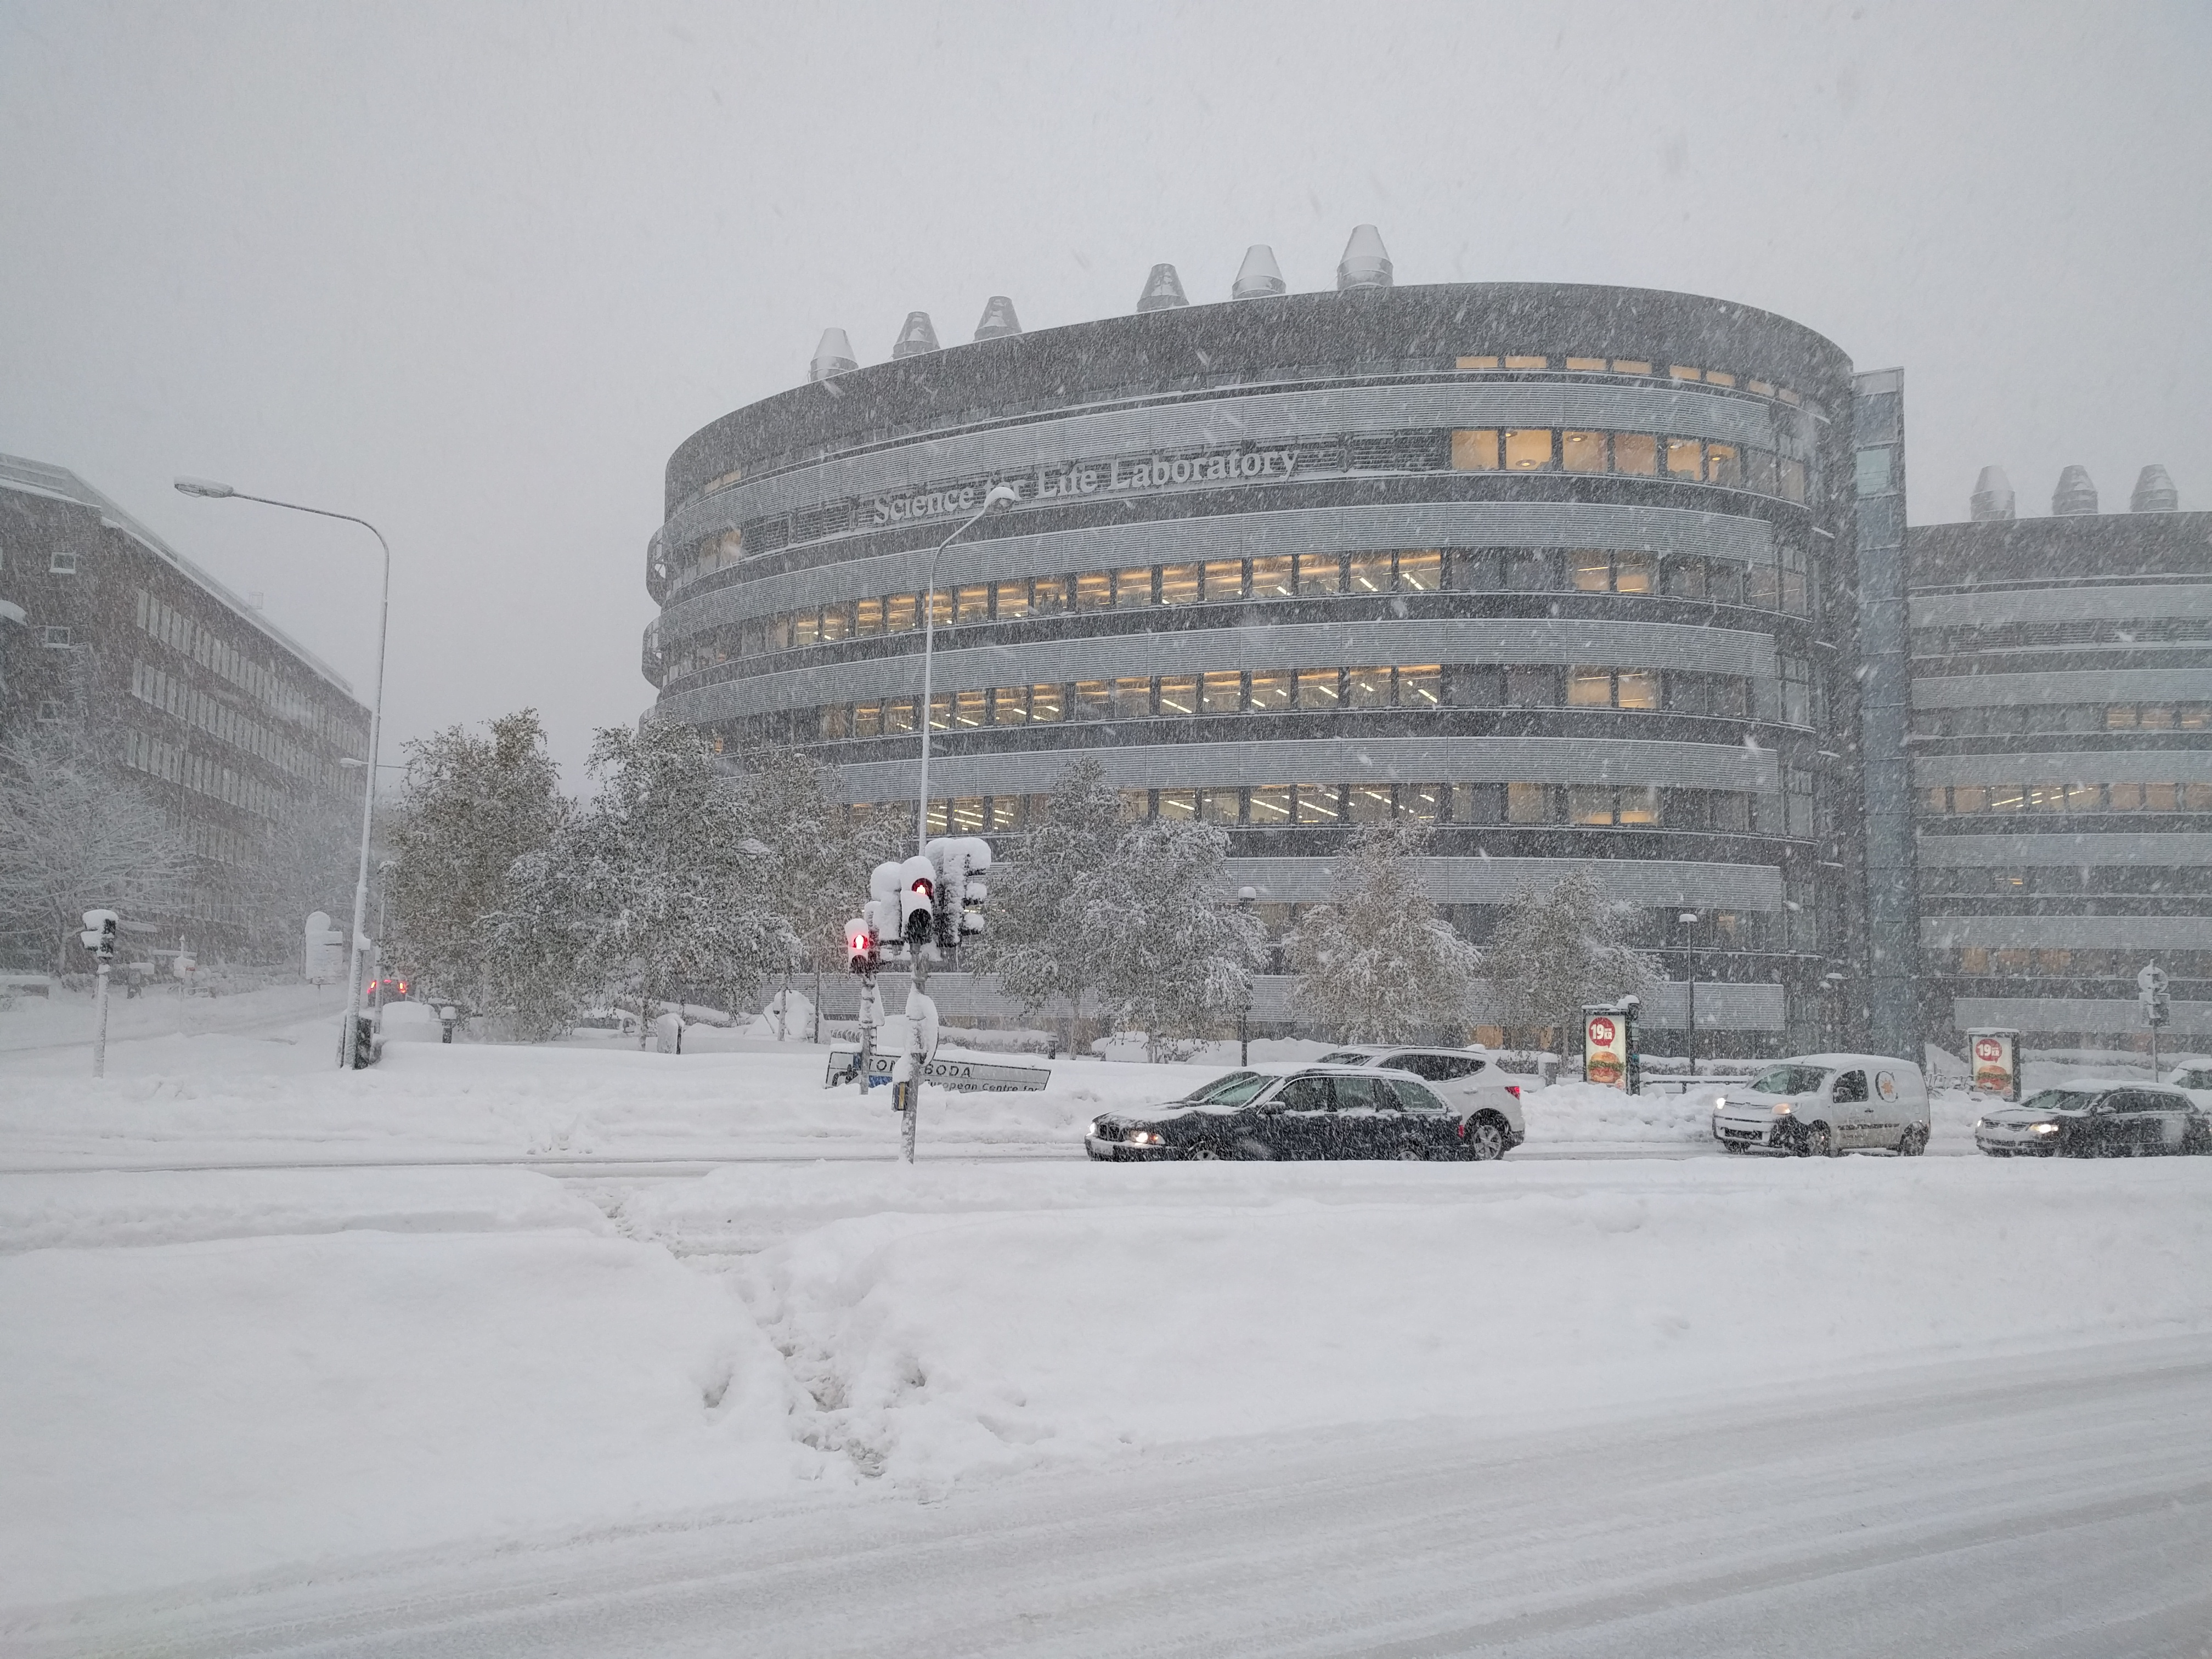
\includegraphics[width=\paperwidth]{pictures/Snowpocalypse-SciLifeLab.jpg}
}

\begin{frame}[plain,noframenumbering]{Any questions?}
\end{frame}

\usebackgroundtemplate{
	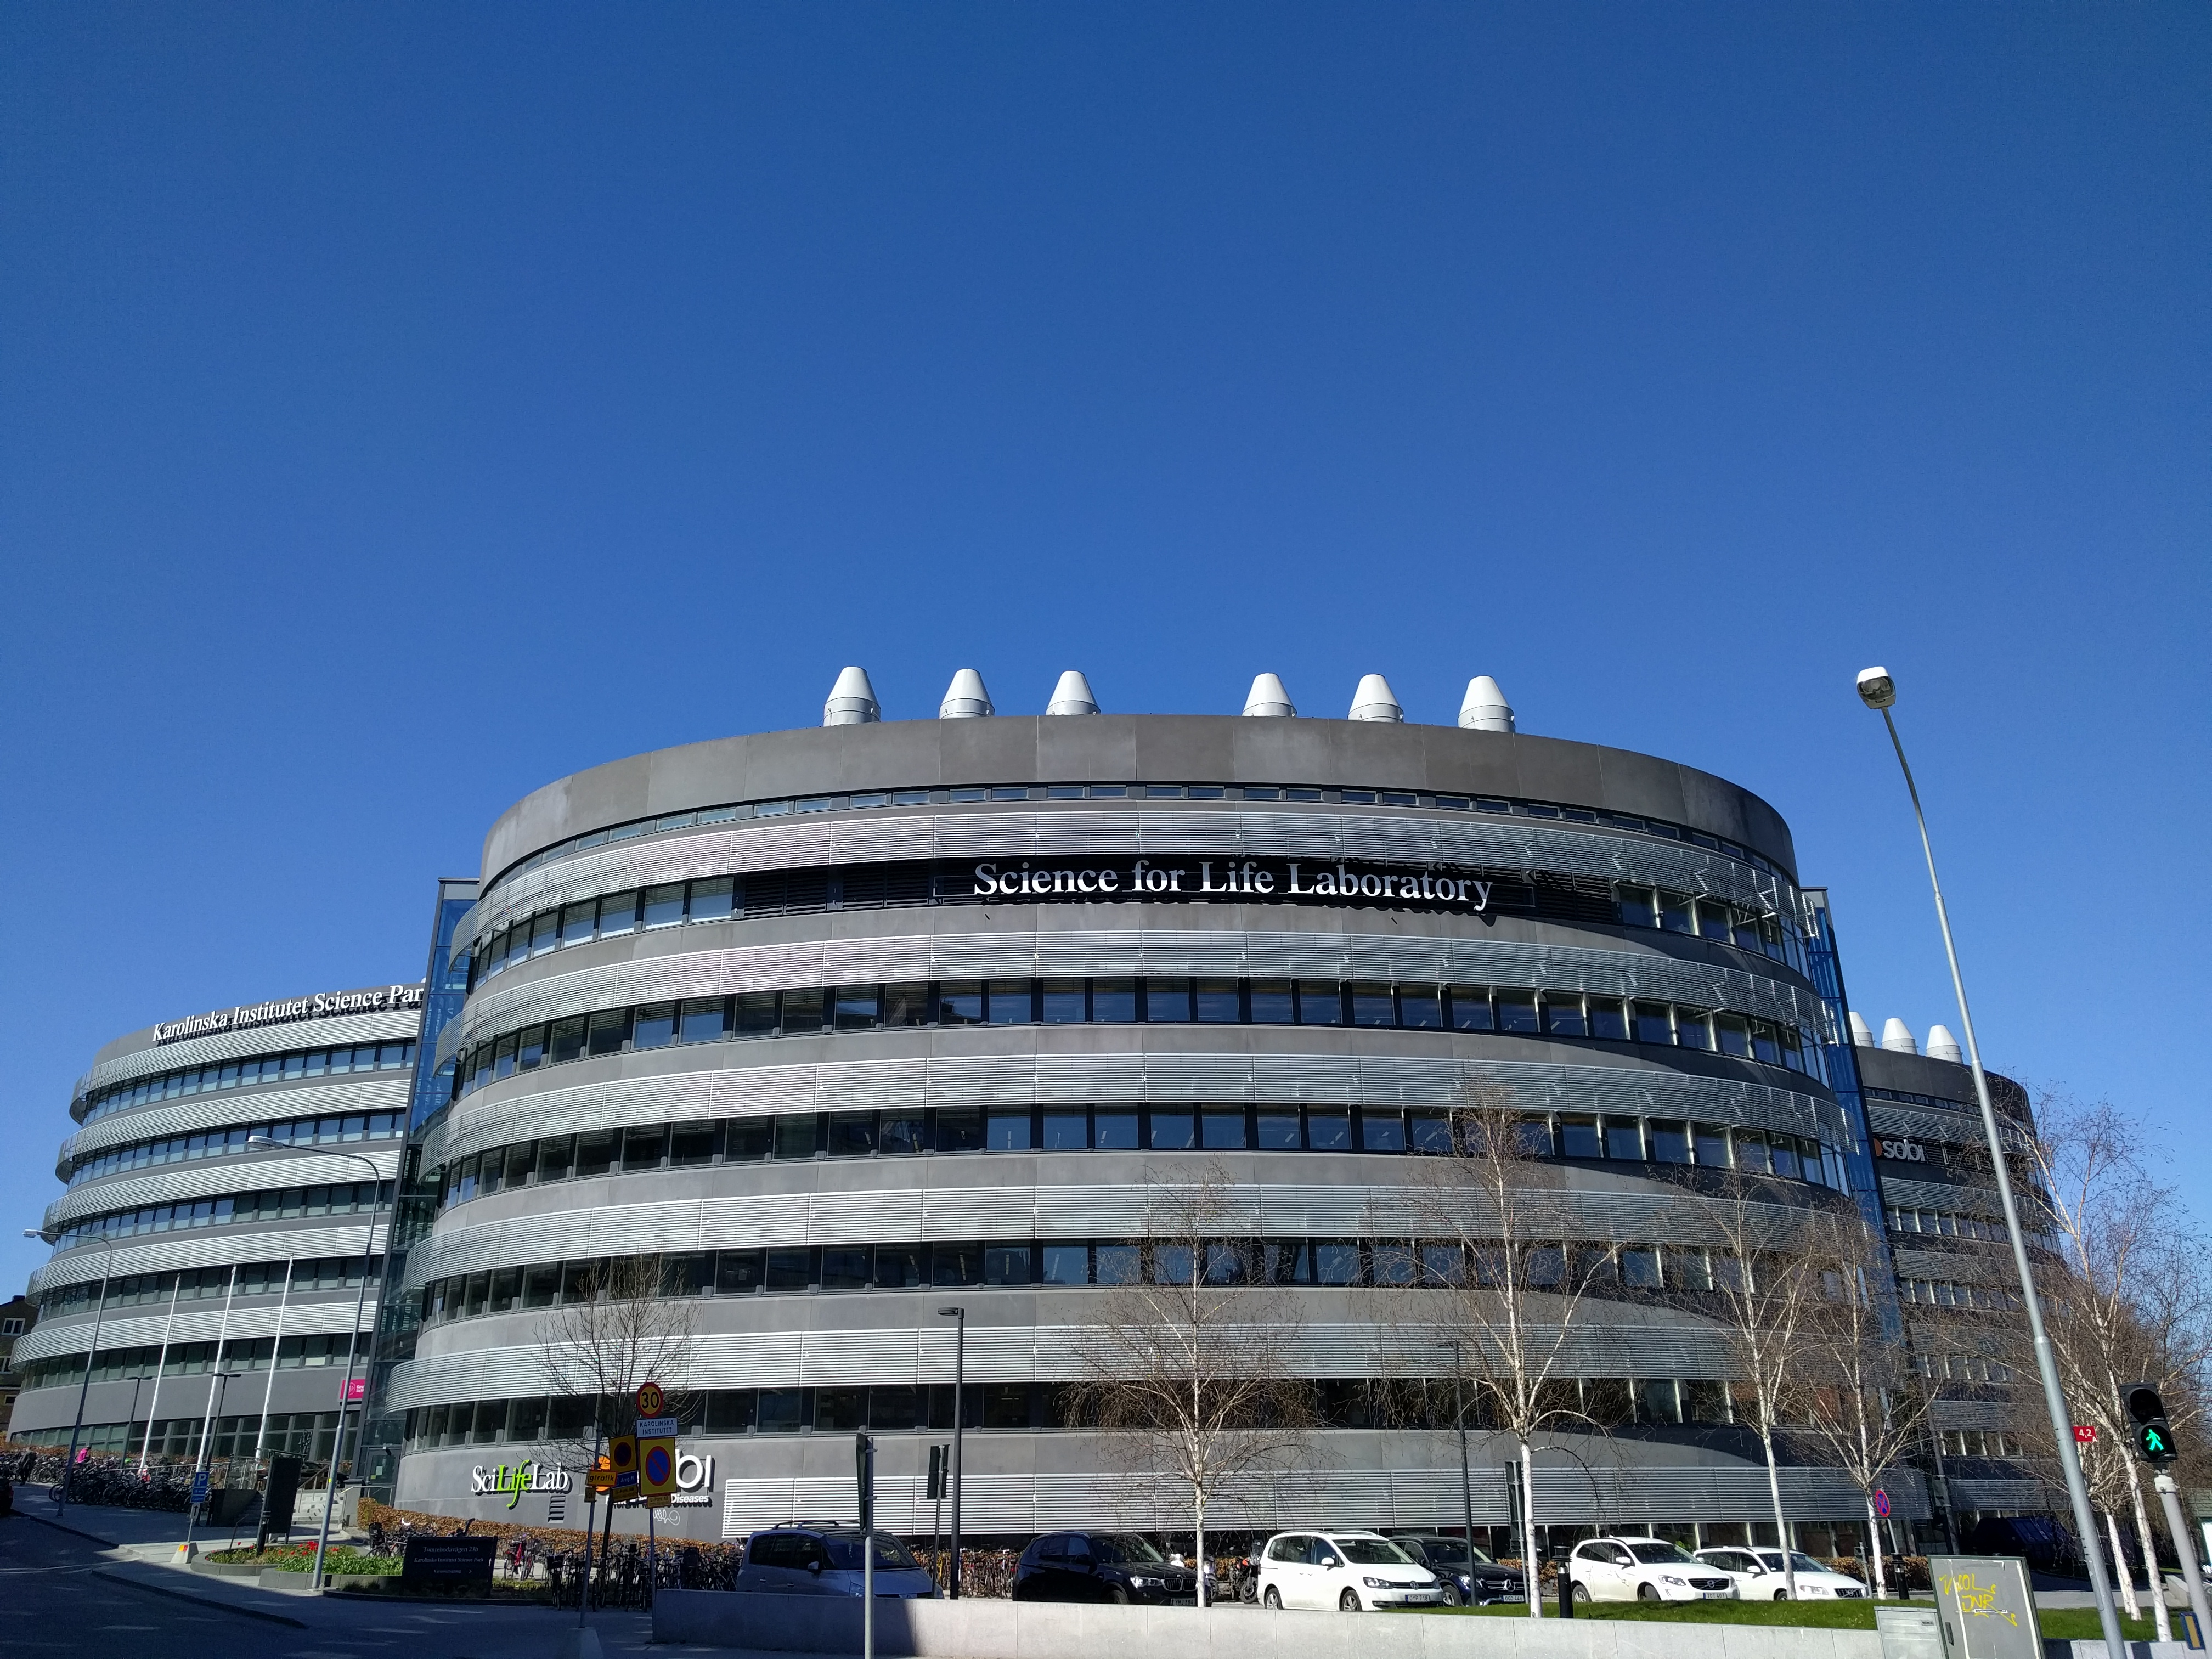
\includegraphics[width=\paperwidth]{pictures/SciLifelab-BlueSky.jpg}
}

\begin{frame}[plain,noframenumbering]{Any questions?}
\end{frame}

\end{document}
